\begin{ledgroupsized}[r]{120mm}%
\footnotesize%
\pstart%
\noindent%
\textbf{\"{U}berlieferung:}%
\pend%
\end{ledgroupsized}%
\begin{ledgroupsized}[r]{114mm}%
\footnotesize%
\pstart%
\parindent -6mm%
\makebox[6mm][l]{\textit{E}}%
Aufzeichnung:
\cite{01152}\glqq Manuscrit inédit de Leibniz. Les plans de l'achèvement du Louvre et la pyramide triomphale de Perrault\grqq,
hrsg. von \textsc{L.A. Foucher de Careil},
\textit{Journal g\'{e}n\'{e}ral de l'instruction publique et des cultes} XXVI, Nr.~32 (22. April 1857), S.~235f.
Foucher de Careil soll laut eigener Angabe das Manuskript
dieser Aufzeichnung in einer \textit{bibliothèque d'Allemagne} gefunden haben
(siehe ebd., S.~235).
Das Manuskript gilt heute als verschollen.%
\newline%
Cc 2, Nr. 00%
\pend%
\end{ledgroupsized}%
%
\vspace*{5mm}%
\begin{ledgroup}%
\footnotesize%
\pstart%
\noindent%
\footnotesize{%
\textbf{Datierungsgr\"{u}nde:}
Leibniz gibt als Datum des Gespr\"{a}chs den 22. Januar an, ohne das Jahr zu erwähnen.
Im Text wird aber von einer 1675 signierten Wandtafel berichtet, die auf Colberts Funktion als Generalleiter des Louvre-Bauwerks anspielt
(siehe unten, S.~\refpassage{RK56900_z1}{RK56900_z2}).
Das Gespr\"{a}ch fand folglich aller Wahrscheinlichkeit nach am 22. Januar 1676 statt.
}%
\pend%
\end{ledgroup}%
%
%
\vspace*{8mm}%
\count\Bfootins=1200
\count\Cfootins=1200
\count\Afootins=1200
\pstart%
\normalsize%
\noindent%
% [235]
[p.~235] Mons. Perrault,\protect\index{Namensregister}{\textso{Perrault}, Claude 1613-1688}
le medecin de l'Academie royale des sciences,\protect\index{Sachverzeichnis}{Academie royale des sciences}
auteur du \edtext{Vitruve\protect\index{Namensregister}{\textso{Vitruvius} Pollio, Marcus ca 70-10 v.Chr.} francois,}{\lemma{Vitruve  francois}\Cfootnote{\cite{01014}\textsc{Vitruvius}, \textit{Les dix livres d'architecture, corrigez et traduits nouvellement en François, avec des Notes et des Figures}, hrsg. von \textsc{C.~Perrault}, Paris 1673.}}
%
m'a cont\'{e} aujourd'hui (22 janvier) quantit\'{e} de choses remarquables touchant le bastiment du Louvre.\protect\index{Ortsregister}{Louvre}
Mons. Colbert,\protect\index{Namensregister}{\textso{Colbert}, Charles 1625-1696}
ayant pris la surintendance des bastiments pour achever le Louvre,\protect\index{Ortsregister}{Louvre}
fit faire des desseins par les habiles architectes de France.\protect\index{Ortsregister}{Frankreich}
Mons. de Veau\protect\index{Namensregister}{\textso{Le Vau}, Louis 1612-1670}
premier architecte du roy,\protect\index{Namensregister}{\textso{Ludwig XIV}., roi de France 1643-1715}
en donna un comme pour servir de base; les autres le controlerent, firent des remarques l\`{a} dessus et donn\`{e}rent leur dessein.
Mons. Colbert\protect\index{Namensregister}{\textso{Colbert}, Charles 1625-1696} en tira de luy même l'essence, ayant \'{e}crit 4 feuilles d'ecriture menue de sa main pour en faire rapport au roy.\protect\index{Namensregister}{\textso{Ludwig XIV}., roi de France 1643-1715}
Mons. Perrault,\protect\index{Namensregister}{\textso{Perrault}, Charles 1628-1703}
fr\`{e}re du medecin, qui est à present le controlleur general des bastimens et jardins\protect\index{Sachverzeichnis}{jardin} de France\protect\index{Ortsregister}{Frankreich}
(il y en a 4 qui servent par quartier),
et qui exerce sous Mons. Colbert\protect\index{Namensregister}{\textso{Colbert}, Charles 1625-1696}
l'intendance des bastimens etait en ce temps connu de Mons. Colbert\protect\index{Namensregister}{\textso{Colbert}, Charles 1625-1696}
et prestait la plume à une Academie des belles lettres dont Mons. Colbert\protect\index{Namensregister}{\textso{Colbert}, Charles 1625-1696}
\'{e}tait le protecteur et de la quelle estaient
Monsieu Chapelain\protect\index{Namensregister}{\textso{Chapelain}, Jean 1595-1674}
scavantissime pour le grec et qui a
\edtext{traduit Xenophon,\protect\index{Namensregister}{\textso{Xenophon} ca. 430-354 v.Chr.}}{\lemma{traduit Xenophon}\Cfootnote{\cite{00357}\textsc{Xenophon}, \textit{La Cyrop\'{e}die}, hrsg. von \textsc{F.~Charpentier}, Paris 1661.}}
Mons. Charpentier\protect\index{Namensregister}{\textso{Charpentier}, Francois 1620-1702} et quelques autres. Mons. Perrault\protect\index{Namensregister}{\textso{Perrault}, Charles 1628-1703} y faisant fonction de secretaire, o\`{u} l'on travaille à des medailles, devises et autres choses pour la gloire du roy\protect\index{Namensregister}{\textso{Ludwig XIV}., roi de France 1643-1715}, il dit à son frere le medecin pourquoy il ne faisait pas aussi quelque dessein luy qui avoit travaillé longtemp à l'architecture\protect\index{Sachverzeichnis}{architecture}; il s'en defendit, mais à la fin il en fit un; il desseigna d'une maniere douce et agreable bien qu'en ce temps les architectes ne desseignait pas si bien et n'achevait pas, n'y finissait pas, se contentant de leurs traits et de donner les ombres par leur marche de lavis.
Mons. Perrault\protect\index{Namensregister}{\textso{Perrault}, Charles 1628-1703} le controlleur ayant montr\'{e} ce dessein à Mons. Colbert,\protect\index{Namensregister}{\textso{Colbert}, Charles 1625-1696}
il luy plut fort et Mons. le Brun\protect\index{Namensregister}{\textso{Le Brun}, Charles 1619-1690} qui avait m\'{e}pris\'{e} tous les autres s'arresta fort à celuy-ci.
Mons. Colbert\protect\index{Namensregister}{\textso{Colbert}, Charles 1625-1696} demandant de qui il estoit,
il luy dit qu'il estoit de son fr\`{e}re dont Mons. Colbert\protect\index{Namensregister}{\textso{Colbert}, Charles 1625-1696} demanda qu'il le vint trouver, luy montra tous les autres desseins et les lui donna avec les ecrits et avec le sien qu'il en avait tir\'{e} pour luy en dire son sentiment.
Mons. Perrault\protect\index{Namensregister}{\textso{Perrault}, Claude 1613-1688} fit un
\edtext{petit trait\'{e}}{\lemma{petit trait\'{e}}\Cfootnote{Dem Titel nach ist unter Perraults veröffentlichten Schriften keine anzutreffen, die sich mit den Arbeiten am Louvre befasst.%
%Vielmehr scheint es sich um ein Architektengutachten für Colbert gehandelt zu haben.
}}
o\`{u} il establit des maximes et une espece de systeme; il remarqua les defauts de tous les desseins, et fit voir qu'il y avoit remedi\'{e} avant que de voir les autres desseins. Mons. Colbert\protect\index{Namensregister}{\textso{Colbert}, Charles 1625-1696} en fut fort satisfait. Et on estoit sur le point de s'y arrester. Mais il arriva une chose qui pensa renverser tout. Car Mons.  Colbert\protect\index{Namensregister}{\textso{Colbert}, Charles 1625-1696} considerant les fautes que tant d'architectes francais avaient fait, et qu'un m\'{e}decin leur avait fait la barbe, se mit en teste qu'il fallut que sous ces gens fussent des ignorants et qu'il fallait consulter aussi des architectes \'{e}trangers. On parla au nonce pour \'{e}crire \`{a} Bernini\protect\index{Namensregister}{\textso{Bernini}, Gian Lorenzo 1598-1680}; on luy envoya le plan du Louvre\protect\index{Sachverzeichnis}{Louvre} avec ce qui estoit deja et toutes les sujections, et on luy demanda son avis pour la mani\`{e}re de l'achever. Bernini\protect\index{Namensregister}{\textso{Bernini}, Gian Lorenzo 1598-1680}, au lieu d'envoyer un dessein du Louvre\protect\index{Sachverzeichnis}{Louvre} comme il pouvait estre perfectionn\'{e}, envoya un dessein d'un palais tout nouveau, ce qu'on ne voulait, et s'excusa qu'il ne pouvait pas juger du Louvre\protect\index{Sachverzeichnis}{Louvre} sans l'avoir bien veu. \edtext{Enfin on le fit venir avec grand peine et frais.}{\lemma{Enfin [...] frais}\Cfootnote{Gian Lorenzo Bernini reiste nach Paris Ende April 1665 und hielt sich dort bis Mitte Oktober desselben Jahres auf.}} Mons. Colbert\protect\index{Namensregister}{\textso{Colbert}, Charles 1625-1696} cependant ne parloit plus à Mr Perrault\protect\index{Namensregister}{\textso{Perrault}, Claude 1613-1688} de cette affaire, et gagn\'{e} par les fanfaronnades de Bernini\protect\index{Namensregister}{\textso{Bernini}, Gian Lorenzo 1598-1680}, arresta tout avec luy suivant son dessein.%
\pend%
\pstart%
Bernini\protect\index{Namensregister}{\textso{Bernini}, Gian Lorenzo 1598-1680}, apr\`{e}s avoir receu de grands pr\'{e}sents, et ayant compt\'{e} plus de 50,000 \'{e}cus, s'en retourna, ayant laiss\'{e} un certain Matheo Masthei\protect\index{Namensregister}{\textso{Masthei??}, Matheo?? ??}, architecte tr\`{e}s habile pour conduire l'execution du bastiment. Bernini\protect\index{Namensregister}{\textso{Bernini}, Gian Lorenzo 1598-1680} estoit deja de 80 ans, il n'estoit pas effectivement un architecte si consomm\'{e} qu'il se vantait. Son dessein estoit plein de fautes assez grossieres. Quand il estoit à Paris\protect\index{Ortsregister}{Paris}, il meprisoit tout ce qu'on luy monstroit, il trouvoit miserable tout ce que les Francois avoient fait. Et quand il voyoit un tableau ou une statue d'un Italien, ou antique il s'y arrestoit. Cependant Messieurs Perrault\protect\index{Namensregister}{\textso{Perrault}, Claude 1613-1688}\protect\index{Namensregister}{\textso{Perrault}, Charles 1628-1703} estoient bien mortifi\'{e}s de se voir ainsi rebut\'{e}s; ils prirent la resolution de faire voir par un memoire \`{a} Mons. Colbert\protect\index{Namensregister}{\textso{Colbert}, Charles 1625-1696} non seulement les defauts du dessein de Bernini\protect\index{Namensregister}{\textso{Bernini}, Gian Lorenzo 1598-1680}, mais son adresse ou plustot sa malice, par la quelle il pr\'{e}tendoit d'engager le roy\protect\index{Namensregister}{\textso{Ludwig XIV}., roi de France 1643-1715} si avant insensiblement, qu'on seroit oblig\'{e} à la fin d'abattre le Louvre\protect\index{Sachverzeichnis}{Louvre} et de le faire tout de nouveau; car outre qu'il faisoit faire un mur par dedans qui cachoit l'architecture\protect\index{Sachverzeichnis}{architecture} du Louvre\protect\index{Sachverzeichnis}{Louvre} comme il estoit, il avoit fait tout en sorte que le nouveau bastiment avoit des vides où le vieux avoit des yeux ou fenetres. Ainsi on auroit trouv\'{e} en executant son dessein qu'il falloit abattre tout; ce qui auroit degout\'{e} tout le monde et le roy\protect\index{Namensregister}{\textso{Ludwig XIV}., roi de France 1643-1715} m\^{e}me, et on l'auroit laiss\'{e} l\`{a} entierement, peut etre même que cela estoit un effet de la jalousie italienne qui enviait à la France\protect\index{Ortsregister}{Frankreich} un bastiment aussi prodigieux que le Louvre\protect\index{Sachverzeichnis}{Louvre}; car estant abattu il auroit peut etre jamais est\'{e} rebasti. Mons. Colbert\protect\index{Namensregister}{\textso{Colbert}, Charles 1625-1696} ayant leu et bien consider\'{e} ce memoire, fit venir Matheo Masthei\protect\index{Namensregister}{\textso{Masthei??}, Matheo?? ??} et le questionna sur certains points ou faits qui estoient allegu\'{e}s dans ce memoire; et trouvant qu'il les avouoit, Mons. Colbert\protect\index{Namensregister}{\textso{Colbert}, Charles 1625-1696} dit il est assez. Quelques jours apr\`{e}s le modelle qui se voit encore au Louvre\protect\index{Sachverzeichnis}{Louvre} fut achev\'{e} et le roy\protect\index{Namensregister}{\textso{Ludwig XIV}., roi de France 1643-1715} vint avec toute la cour pour le voir. Mons. Colbert\protect\index{Namensregister}{\textso{Colbert}, Charles 1625-1696} se hasta pour s'y trouver avant le roy\protect\index{Namensregister}{\textso{Ludwig XIV}., roi de France 1643-1715}. Le roy\protect\index{Namensregister}{\textso{Ludwig XIV}., roi de France 1643-1715} vint un moment après. Mons. Colbert\protect\index{Namensregister}{\textso{Colbert}, Charles 1625-1696} le tira à cost\'{e} et luy conta toute l'histoire en luy faisant voir les raisons. Cependant toute la cour regardait le modelle et disoit, voila qui est beau, parce qu'il falloit attendre que le roy\protect\index{Namensregister}{\textso{Ludwig XIV}., roi de France 1643-1715} eust parl\'{e}. Le roy\protect\index{Namensregister}{\textso{Ludwig XIV}., roi de France 1643-1715} enfin le voit aussi, il ne dit mot pour le louer ni pour le censurer, se contentant de questionner Mattheo sur l'effet que tout devoit faire. Le lendemain, Mattheo fut bien surpris de se voir congedi\'{e} avec tous ses murasori. On le recompensa et on le paya fort honnestement. Ces Italiens estant partis, Mons. Colbert\protect\index{Namensregister}{\textso{Colbert}, Charles 1625-1696} dit nous voila seuls. Comment ferons nous. On offrit Mons. Perrault\protect\index{Namensregister}{\textso{Perrault}, Claude 1613-1688} le medecin la charge de premier architecte du roy\protect\index{Namensregister}{\textso{Ludwig XIV}., roi de France 1643-1715}, car on n'estoit point satisfait de Mons. de Veau\protect\index{Namensregister}{\textso{Le Vau}, Louis 1612-1670}. Il refusa et il dit qu'il n'estoit pas architecte de profession et qu'il ne vouloit pas non plus abandonner toute autre chose pour l'amour de l'architecture\protect\index{Sachverzeichnis}{architecture}. Il proposa qu'on establit plustot un conseil d'architecture\protect\index{Sachverzeichnis}{architecture} pour cet effect, sous la direction de Mons. Colbert\protect\index{Namensregister}{\textso{Colbert}, Charles 1625-1696} dont il seroit. Cela fut fait, Mons. Perrault\protect\index{Namensregister}{\textso{Perrault}, Claude 1613-1688} Mons. Le Brun\protect\index{Namensregister}{\textso{Le Brun}, Charles 1619-1690} et M. Veau\protect\index{Namensregister}{\textso{Le Vau}, Louis 1612-1670} et quelques autres en estoient. Ils ne pouvoient s'accorder sur le dessein.
\pend%
\pstart%
Enfin Mon. de Veau\protect\index{Namensregister}{\textso{Le Vau}, Louis 1612-1670} abandonna le sien et consentit à celuy de Mons. Perrault\protect\index{Namensregister}{\textso{Perrault}, Claude 1613-1688} de sorte qu'il n'y avait que deux qui restaient à comparer, celuy de Mons. Perrault\protect\index{Namensregister}{\textso{Perrault}, Claude 1613-1688} et celuy de Mons. le Brun\protect\index{Namensregister}{\textso{Le Brun}, Charles 1619-1690}. On les fit desseigner tout deux par un m\^{e}me peintre d'une même grandeur. Chacun donna ses raisons par escrit. Le roy\protect\index{Namensregister}{\textso{Ludwig XIV}., roi de France 1643-1715} (suivant le sentiment de Mons. Colbert\protect\index{Namensregister}{\textso{Colbert}, Charles 1625-1696}) prefera celuy de Mons. Perrault\protect\index{Namensregister}{\textso{Perrault}, Claude 1613-1688}. Ayant fait examiner tous deux en plein conseil, en pr\'{e}sence de Monsieur, frere du roy\protect\index{Namensregister}{\textso{Philippe d'Orl{´e}ans}, 1640-1701}, mons. le prince et les conseillers d'Estat. Et c'est ce dessein sur le quel on travaille à present. Il y a le devant du Louvre\protect\index{Sachverzeichnis}{Louvre}; il pensait le quarr\'{e} dont le commencement du cost\'{e} de la riviere\protect\index{Ortsregister}{Seine} sera l'appartement de service de la reine; sur le devant même l'appartment de ceremonie de la reine; plus bas du cost\'{e} de la rivi\`{e}re\protect\index{Ortsregister}{Seine} sera l'appartement de service du roy\protect\index{Namensregister}{\textso{Ludwig XIV}., roi de France 1643-1715} de sorte que l'appartement de service du roy\protect\index{Namensregister}{\textso{Ludwig XIV}., roi de France 1643-1715} et de la reine sont tourn\'{e}s vers le midi\protect\index{Sachverzeichnis}{midi}, car le roy\protect\index{Namensregister}{\textso{Ludwig XIV}., roi de France 1643-1715} demeure principalement à Paris l'hyver\protect\index{Sachverzeichnis}{hyver} et par consequent le midy\protect\index{Sachverzeichnis}{midi} est le plus agreable en hyver\protect\index{Sachverzeichnis}{hyver}.%
\pend%
\count\Bfootins=1400
\count\Cfootins=1400
\count\Afootins=1200
\newpage
%\vspace{2ex}% PR: Rein provisorisch !!!
\pstart%
\noindent%
\centering%
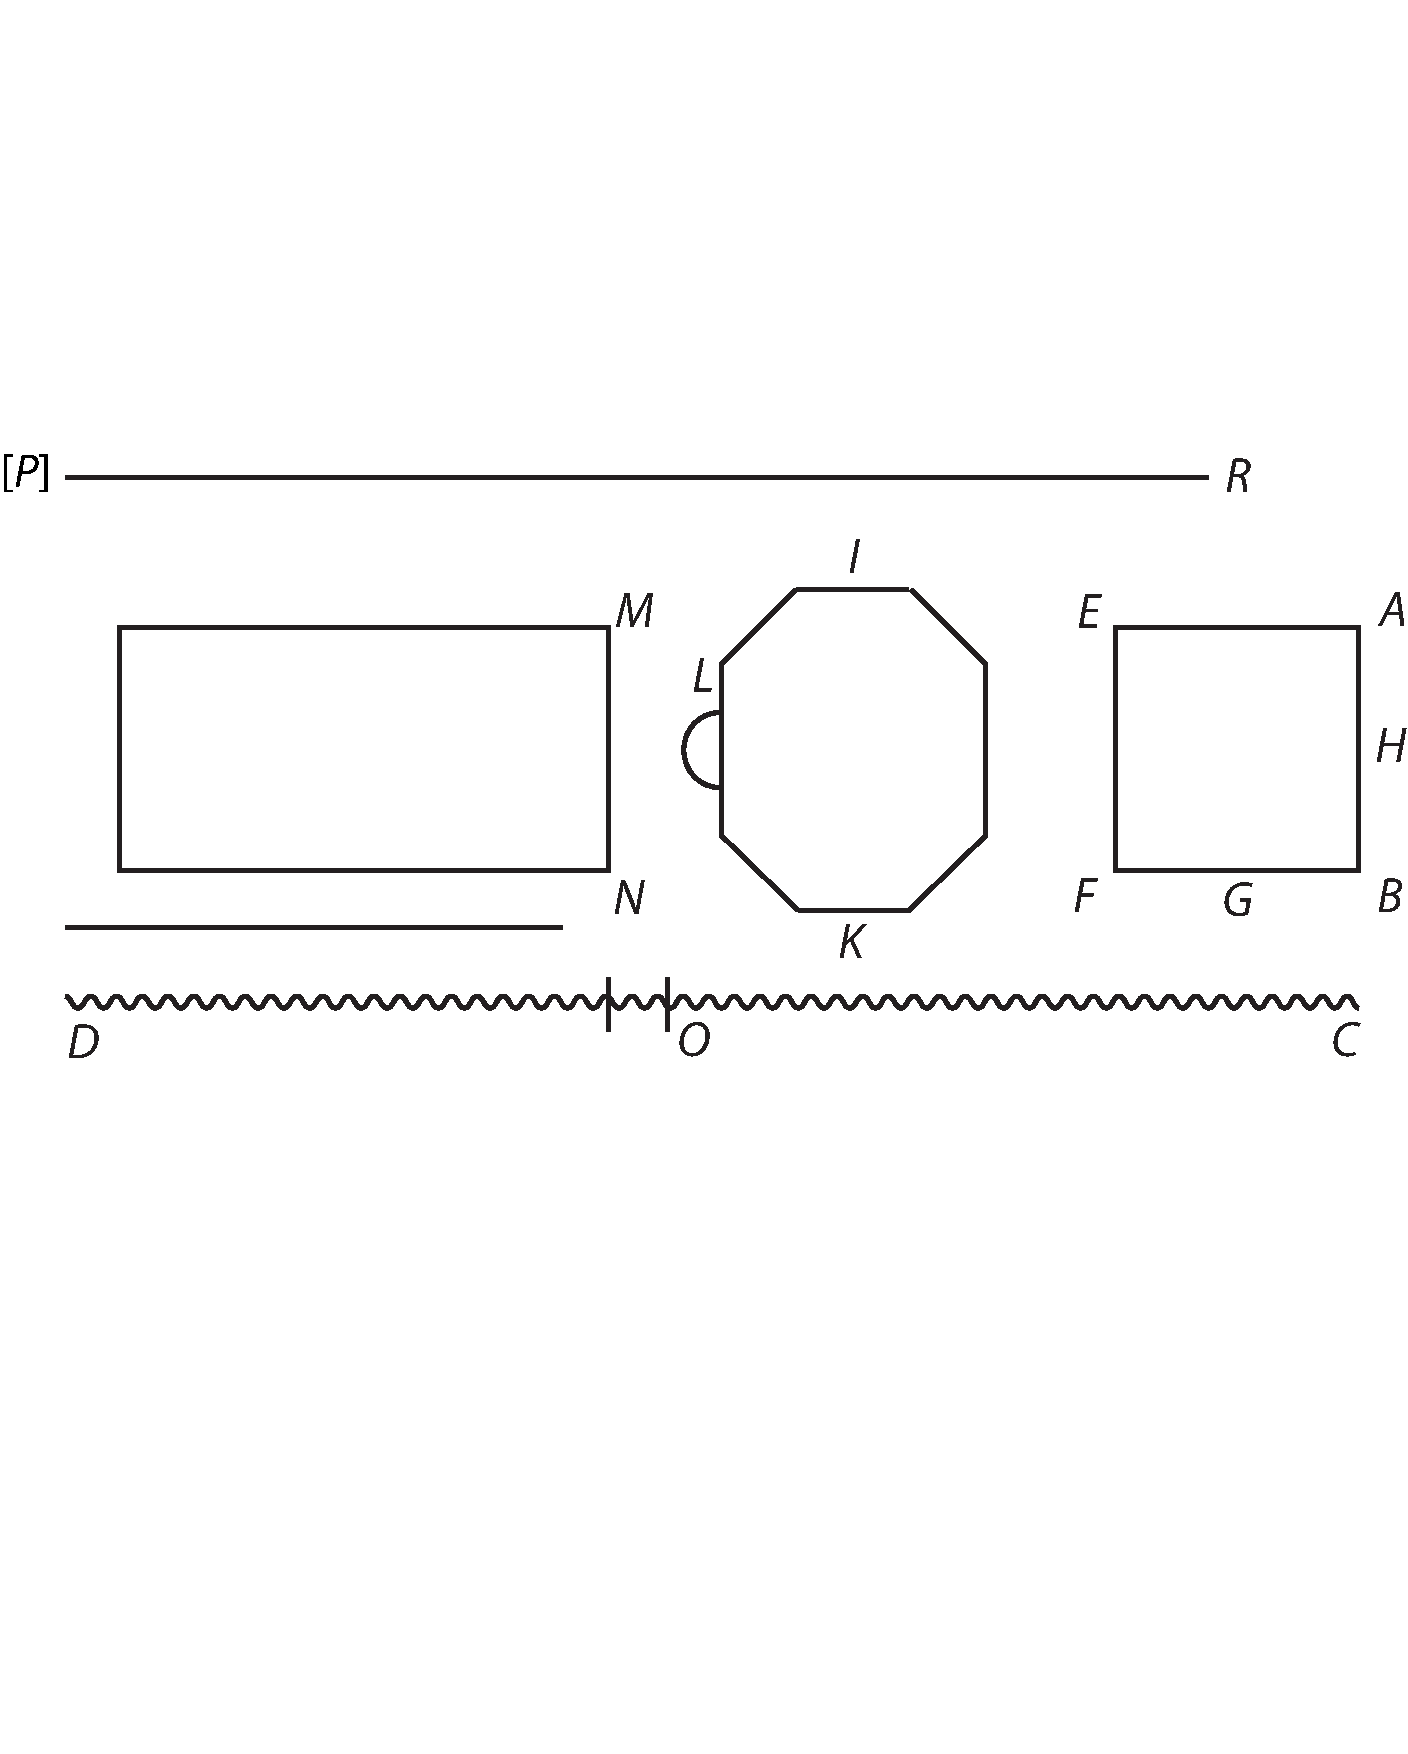
\includegraphics[width=0.75\textwidth]{images/RK56900_235-d1.pdf}%
\edtext{}{\lemma{\hspace*{1,7mm}\lbrack\textit{Fig. 1}\rbrack} \killnumber\Bfootnote{$P$ \textit{erg. Hrsg.}}}\\
\centering [\textit{Fig. 1}]%
\edtext{}{\lemma{\hspace*{1,7mm}\lbrack\textit{Fig. 1}\rbrack}\killnumber\Cfootnote{Zur Abbildung % \lbrack\textit{Fig. 1}\rbrack\ 
findet sich in \textit{E} folgende Bemerkung:
\textit{Nous ferons remarquer que les lettres de renvoi du manuscrit ne sont pas toutes reproduites sur le plan; mais les indications sont suffisantes pour reconnaitre la disposition.}}} 
\pend%
\vspace*{1em}% 
\pstart%
%\noindent%
$AB$ \setline{1}devant du Louvre\protect\index{Sachverzeichnis}{Louvre}, $CD$ courant de la rivi\`{e}re de Seine\protect\index{Ortsregister}{Seine}, $ABEF$ quarr\'{e} du Louvre\protect\index{Sachverzeichnis}{Louvre}, $FG$ appartement de service du roy\protect\index{Namensregister}{\textso{Ludwig XIV}., roi de France 1643-1715}, $GB$ appartement de service de la Reine, $BH$ appartement de ceremonie de la reine, $EF$ sale des soir\'{e}es en bas, gardes en haut, dans les coins l'aile est soutenue de colonnes. $IK$ octogone\protect\index{Sachverzeichnis}{octogone} sale d'audience\protect\index{Sachverzeichnis}{salle d'audience}, etc: il y aura une salle d'une prodigieuse grandeur, $L$ chapelle\protect\index{Sachverzeichnis}{chapelle} dont un dome comme le val de Grace mais plus grand.
Ce sera comme la paroisse du Louvre:\protect\index{Sachverzeichnis}{Louvre} $MN$ rue qui separe les Tuileries\protect\index{Ortsregister}{Tuileries} du Louvre:\protect\index{Sachverzeichnis}{Louvre} 
$N$ porte, $O$ pont de pierre sur la rivi\`{e}re:\protect\index{Ortsregister}{Seine}
$MN$ bibliotheque\protect\index{Sachverzeichnis}{bibliotheque du roi} du roy\protect\index{Namensregister}{\textso{Ludwig XIV}., roi de France 1643-1715} \`{a} main droite, un peu à cost\'{e} salle des peintures:\protect\index{Sachverzeichnis}{salle des peintures}
$MNP$ Tuileries:\protect\index{Ortsregister}{Tuileries}
$PR$ rue St Honore: la ligne $PR$ des 700 toises. [p.~236]%
\pend%
\pstart%
Mons. Perrault\protect\index{Namensregister}{\textso{Perrault}, Claude 1613-1688} le medecin est aussi auteur du dessein de l'arc triomphal, il en avait fait plusieurs; on en choisit celuy qui cousta le moins. Il avait propos\'{e} une belle pyramide toute massive, perc\'{e}e par dedans d'un escalier etroit qui tourne en vis jusqu'en haut. Il y aura en haut un globe de cuivre de trois toises de diametre tout massif, la hauteur sera deux fois celle de la tour de Nostre Dame. Il me montra des devises pour les 4 faces qui representeront les 4 parties du monde, un aigle regardat le soleil avec ces mots \textso{me sustinet unus!} pour l'Europe\protect\index{Ortsregister}{Europa} pour signifier l'Empereur seul capable de regarder ce soleil. Cela est aussi honorable à l'empereur qu'au roy\protect\index{Namensregister}{\textso{Ludwig XIV}., roi de France 1643-1715}. Asie\protect\index{Ortsregister}{Asien} repr\'{e}sent\'{e}e par un phenix qui signifie l'Empire ottoman\protect\index{Ortsregister}{Osmanisches Reich} avec ce mot:
\textso{me suspicit unum.}
\textso{Afrique}\protect\index{Ortsregister}{Afrika} par \makebox[1.0\textwidth][s]{un Elephant qui salue le soleil (Roy d'Ardres). \textso{Amerique}\protect\index{Ortsregister}{Amerika} par un dragon, \textso{draco}}
\pend
\newpage
\pstart\noindent \textso{Hesperidum pomis sive auro incubans}, avec ce mot \textso{quas servat mihi debet opes, debet soli qui produxit, id est in Galliam\protect\index{Ortsregister}{Frankreich}}\textso{ omnes America\protect\index{Ortsregister}{Amerika}}\textso{ divitiae transfunduntur praeter regis destinata in Americam\protect\index{Ortsregister}{Amerika}}. Mons. Perrault\protect\index{Namensregister}{\textso{Perrault}, Claude 1613-1688} me montra encore quantit\'{e} d'autres devises de la facon, comme:
\textso{Dum ludit metuendus,} Mons. le Dauphin. C'est un dauphin qui joue dans les vagues et qui est \textso{praenuntio tempestatis} pour dire que Mons. le dauphin est deja à craindre aux ennemis de la France\protect\index{Ortsregister}{Frankreich} quoiquil ne paraisse qu'enfant et innocent. On a mis cette devise sur les banderoles du regiment des gardes des Mons. le Dauphin. \textso{Inspiciendo} une devise où il n'y a qu'une autruche qui ne fait eclore qu'avec ses yeux en regardant fixement comme les naturalistes\protect\index{Sachverzeichnis}{naturalistes} rapportent. Cette devise est pour Mons. Colbert\protect\index{Namensregister}{\textso{Colbert}, Charles 1625-1696} comme surintendant. \textendash\ \textso{Je ne brusle que pour la guerre}, une meche allum\'{e}e signifie M. le duc de Longueville\protect\index{Namensregister}{\textso{Charles-Paris d'Orl\'{e}ans-Longueville} 1649-1672}, celuy qui fut tu\'{e} au passage du Rhin\protect\index{Ortsregister}{Rhein}. \textso{Ducendis Regibus aptae} pour l'abb\'{e} de Beaumont\protect\index{Namensregister}{\textso{Beaumont}, Vincent Ragot de 1624-1714} precepteur du roy\protect\index{Namensregister}{\textso{Ludwig XIV}., roi de France 1643-1715} par apr\`{e}s archeveque de Paris\protect\index{Ortsregister}{Paris} qui avoit 7 etoiles dans ses armes. L'allusion est aux trois rois de l'Orient que l'Etoile menoit. \textso{Il ne cache point ma flamme}, une Etne\protect\index{Ortsregister}{\"{A}tna} qui jette flamme pour une mari\'{e}e qui fait gloire de son amour au lieu que les autres feux sont cach\'{e}s.
\pend%
\count\Bfootins=1200
\count\Cfootins=1200
\count\Afootins=1200
\pstart%
\textso{Devise de l'observatoir:} sic itur ad astra! une lunette d'approche.
\pend%
\pstart%
\textso{Nullum}\edlabel{RK56900_z1}%
\textso{ non moveo lapidem} repr\'{e}sente une grande pierre du Louvre\protect\index{Sachverzeichnis}{Louvre} elev\'{e}e sur une machine: il est souscrit: \textso{prefectus regionum officiorum} 1675 pour dire que c'est mons. Colbert\protect\index{Namensregister}{\textso{Colbert}, Charles 1625-1696} surintendant des bastiments qui fait remuer tout pour le bien du roi et de l'Estat.\edlabel{RK56900_z2}%
\pend%
\pstart%
Il y avoit quantité d'autres de moindre sorte, comme une flamme qui s'eteint estant renvers\'{e}e avec un mot qui dit que le trop grand feu de l'amour s'\'{e}touffe en soy-même. \textendash\ Voicy la devize de Mons. Perrault\protect\index{Namensregister}{\textso{Perrault}, Claude 1613-1688} lui même:
c'est une lanterne sourde avec ce mot: \textso{non ut videor}, parce que la lanterne sourde fait voir les autres sans decouvrir celui qui voit. Cela est pour un philosophe qui se contente de voir clair dans les sciences, et dans les secrets de la nature\protect\index{Sachverzeichnis}{nature}, quoiqu'il ne soit pas veu ny connu.
\pend%
\pstart%
Mons. le Brun\protect\index{Namensregister}{\textso{Le Brun}, Charles 1619-1690} croyoit que le dessein du Louvre\protect\index{Sachverzeichnis}{Louvre} de M. Perrault\protect\index{Namensregister}{\textso{Perrault}, Claude 1613-1688} quoique beau seroit d'une execution tr\`{e}s difficile. Mais Mons. Perrault\protect\index{Namensregister}{\textso{Perrault}, Claude 1613-1688} a trouv\'{e} un tr\`{e}s habile entrepreneur ce me semble Preaux ou Preat qui est admirablement exact, les pierres sont bien taill\'{e}es, tout est avec une beaut\'{e} admirable. Et le roy\protect\index{Namensregister}{\textso{Ludwig XIV}., roi de France 1643-1715} le voyant dit en pr\'{e}sence de plusieurs:
\textit{si Versailles\protect\index{Ortsregister}{Versailles} pouvoit estre basti comme cela.}
On remarqua que le roy\protect\index{Namensregister}{\textso{Ludwig XIV}., roi de France 1643-1715} estoit en quelque facon jaloux de la beaut\'{e} du Louvre\protect\index{Sachverzeichnis}{Louvre}, car il regarde le Louvre\protect\index{Sachverzeichnis}{Louvre} comme le bastiment des rois de France\protect\index{Ortsregister}{Frankreich}, mais Versailles\protect\index{Ortsregister}{Versailles} comme le sien.
\pend%
\count\Bfootins=1500
\count\Cfootins=1500
\count\Afootins=1500
%%%%  PR: Hier endet das Stück.